% 先端芸術音楽創作学会会報テンプレート ver.200908
% By Daichi Ando
% based on ICMC2005

\documentclass{jsarticle}
\usepackage[dvipdfmx]{graphicx}
\renewcommand{\baselinestretch}{0.9}
\usepackage{url}
\usepackage{ascmac}
\usepackage{jssa,amsmath}
\usepackage{mediabb}
\usepackage{listings,jlisting}
\usepackage{plext}
\usepackage{setspace}
\usepackage{color}
\usepackage{setspace}

\definecolor{mygray}{rgb}{0.9,0.9,0.9}

\lstset{%
 backgroundcolor=\color{mygray},
 basicstyle={\small\ttfamily},%
 stringstyle={\small},
 breaklines=true,
 columns=[l]{fullflexible},%
 frame={l},
 numbers=left,%
 tabsize=3,%
 xrightmargin=0zw,%
 xleftmargin=0zw,%
 numberstyle={\scriptsize},%
 stepnumber=1,
 numbersep=1zw,%
 lineskip= -0.5zw%
}

\def\boutenchar{・}
\def\lstlistingname{リスト}

% Title.
% ------
% LaTeX環境によっては,maketitleでエラーが出ることもあるが,強行して良い

\title{Super Collider チュートリアル (4)\\ 
Super Collider Tutorials (4)
}

% Paper Category 論文,報告,連載,書評……など
\category{連載}

% Single address
% To use with only one author or several with the same address
% ---------------
\oneauthor
  {美山 千香士\\Chikashi Miyama} 
  {ケルン音楽舞踏大学\\Hochschule f\"{u}r Musik und Tanz K\"{o}ln} 

\begin{document}

%%% --ページ数等の指定
\makeatletter 
\def\ps@myheadings{% 
\let\ps@jpl@in\ps@plain% 
\def\@evenhead{\reset@font\hfil\leftmark\hfil}% 
\def\@oddhead{\reset@font\hfil\rightmark\hfil}% 
\let\@mkboth\@gobbletwo% 
\let\sectionmark\@gobble% 
\let\subsectionmark\@gobble% 
% 
\def\@oddfoot{\reset@font\hfil-- \thepage --\hfil}% 
\let\@evenfoot\@oddfoot 
} 
\makeatother 

%%% 
%%% 開始ページ数を設定する 
%投稿の段階では無視

\setcounter{page}{ 3 } 
\pagestyle{myheadings} 

%%% 
%%% 論文のVol., No., pp.を設定する 
% 投稿の段階では無視

\markright{\footnotesize \gt 先端芸術音楽創作学会 会報 Vol.1 No.1 pp.9--16 }

%%% 
%%% \maketitleの直後の行に \thispagestyle{myheadings} を挿入する。 

\maketitle
\thispagestyle{myheadings}

%
\begin{abstract}
 本連載では、リアルタイム音響合成環境のSuperCollider(SC)の使い方を、同ソフトを作品創作や研究のために利用しようと考えている音楽家、メディア・アーティストを対象にチュートリアル形式で紹介する。\\
SuperCollider(SC) is a realtime programming environment for audio synthesis. This article introduces SC to musicians and media artists who are planning to utilize the software for their artistic creations and researches.

\end{abstract}
%
\section{今回の目標:SCでエフェクタを作成する}
前回までは、SCを用いて音を生成する方法を学習してきたが、今回はマイクからの入力音をリアルタイムに加工する方法に焦点をあて、リング・モジュレーション、ディストーション、ピッチ・シフター、ディレイ、リバーブなどのエフェクトをSCで作成する。ハウリングを避けるために、本稿のプログラムを実行する際には、ヘッドフォンなどを着用すること。また、OS側の設定で必ずマイクがオーディオの入力機器に選択されていることを事前に確認すること。Macの場合は、マイクを「環境設定」パネルでOSのオーディオ入力デバイスとして設定すると、SCサーバーの起動時にリスト\ref{device_list}のように、マイク入力がリストの最初に列挙される。

\begin{lstlisting}[caption=入出力デバイスのリスト,label=device_list]
Number of Devices: 3
   0 : "Built-in Microph"
   1 : "Built-in Input"
   2 : "Built-in Output"
\end{lstlisting}

\section{マイクからの入力音を得るには}
マイクからの入力をSCで得るには、リスト\ref{code:mic_input}のように{\bf SoundIn}というUgenを用いる.このプログラムで単純にはマイクからの音声をオーディオ出力デバイスに送っている。マイクからの音がそのままヘッドフォンで聞くことができれば成功である。

\begin{lstlisting}[caption=マイク入力,label=code:mic_input]
{
	SoundIn.ar([0,1]);
}.play
\end{lstlisting}

\begin{itembox}[l]{SoundIn}
{\footnotesize 
コンピュータのマイクやサウンドカードからの音声入力を得る。{\it bus}にArrayを与える事で複数のチャンネルの入力を取得することもできる。\\
.ar({\it bus}, {\it mul}, {\it add})\\
{\it bus}$\cdots$入力チャンネル番号。Arrayを与えることで、複数のチャンネルを同時に取得可能。\\
}
\end{itembox}

\section{リング・モジュレーション}

最も単純なエフェクトとして、K・シュトックハウゼンの「マントラ」などで著名なリングモジュレーションを実装する。
このエフェクトはリスト\ref{code:rm}のように、SoundInからの入力音にサイン波を掛けあわせて実現する事ができる。

\begin{lstlisting}[caption=リング・モジュレーション,label=code:rm]
{
	SoundIn.ar([0,1]) * SinOsc.ar(MouseX.kr(20,880));
}.play
\end{lstlisting}

\section{ディストーション}
音信号を増幅し歪ませる事で、豊かな倍音を含んだ太い音を得る、ロック・ギターでお馴染みのディストーションはSC3ではリスト
\ref{code:dst}のように.distortメソッドを用いてプログラムする事ができる。

\begin{lstlisting}[caption=ディストーション, label=code:dst]
{
	SoundIn.ar([0,1], 100).distort /100;
}.play
\end{lstlisting}

ゲインを調整する事で歪みの深さを調整する事も可能である。リストではゲインをSoundInの{\it mul}引数を100に設定して100倍に増幅し、.distortにより歪ませた後、「/ 100」で音量の調整をしている。
この他にも.softclipを使うと.distortと違った歪み方をさせることが可能である。図\ref{fig:comparison}は10倍に増幅したサイン波をそれぞれ.softclipと.distortで歪ませた時の波形の違いを図示したものである。

\begin{figure}[ftbp]
	\begin{center}
		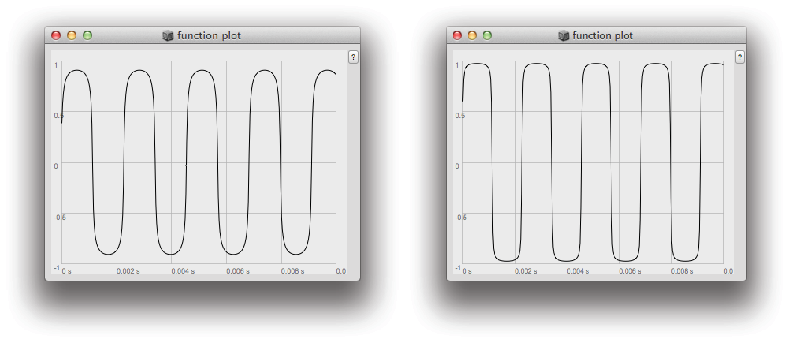
\includegraphics[scale=0.6]{comparison.pdf}
	\end{center}
	\caption{distortion(左)とsoftclip(右)により歪ませた正弦波}
	\label{fig:comparison}
\end{figure}

\section{ピッチ・シフター}
入力音のピッチを自在に変化させるピッチ・シフターは{\bf PitchShift}というUgenを用いれば簡単にプログラム可能である。
過剰に音高を変化させると原音の音色と全く異るものとなるので、原音の音色をなるべく保ちたい場合はあまり極端なパラメータを設定しない方がよい。リスト\ref{code:ps}では{\it pitchRatio}のパラメータを0.5に設定しているため、原音が半分の速度での再生される、このため原音より1オクターブ低くなる。

\begin{lstlisting}[caption=ピッチシフター, label=code:ps]
{
	PitchShift.ar(SoundIn.ar([0,1]), pitchRatio:0.5);
}.play
\end{lstlisting}

例えば、原音より短三度高い音と長三度低い音を付加してピッチシフターを利用して和音を作る事も可能である。このように音階上にピッチシフトを行う場合は、以前に学習した.miditocpsを利用する。

\begin{lstlisting}[caption=ピッチシフターによる和音, label=code:ps_chord]
{
	a = PitchShift.ar(SoundIn.ar([0,1]), pitchRatio: 3.midicps / 0.midicps);
	b = PitchShift.ar(SoundIn.ar([0,1]), pitchRatio: -4.midicps / 0.midicps);
	a+b
}.play
\end{lstlisting}

.midicpsは、MIDIノートナンバーから周波数を出力させるメソッドであり。0.midicpsを実行すると、MIDIノートナンバー「0」の周波数を得られる。MIDIノートナンバー「0」より長三度高い「4」と短三度低い「-3」の周波数をそれぞれもとめ、それを「0」の周波数と比較することで、周波数比を得られる、これを{\it pitchRatio}の値としてPitchShift.arに与える事でピッチシフターを用いた長三和音を作る事ができる。

\begin{itembox}[l]{PitchShift}
{\footnotesize 
ピッチシフトを行うUgen。音程はpitchRatioで指定する。dispersionのパラメータを用いることで、音程のランダマイズなども可能。\\
.ar({\it in}, {\it windowSize}, {\it pitchRatio}, {\it pitchDispersion}, {\it timeDispersion}, {\it mul}, {\it add}, )\\

{\it in}$\cdots$入力信号\\
{\it windowSize}$\cdots$ウインドウ・サイズ\\
{\it pitchRatio} $\cdots$ピッチ・レシオ\\
{\it pitchDispersion} $\cdots$ピッチ分散度\\
{\it timeDispersion} $\cdots$時間分散度\\
}
\end{itembox}

\section{ディレイ}
ここでは入力音を一定時間遅延させ、やまびこのような効果を得るディレイとその応用を数種作成する。

\subsection{シンプルなディレイ}

遅延効果をSCで用いるには{\bf DelayN}というUgenを仕様する。このUgenの第2、第3引数はそれぞれ、最大ディレイ・タイムとディレイタイムで、最大ディレイ・タイムの値を元に、SCはディレイ用のバッファを用意し、それを利用してディレイ・タイムで指定された時間だけ入力音を遅延させて出力する。最大ディレイ・タイムを超えたディレイ・タイムを設定する事はできない\ref{code:delay}。
\begin{lstlisting}[caption=ディレイ, label=code:delay]
{
	DelayN.ar(SoundIn.ar([0,1]), 0.5, 0.5)
}.play
\end{lstlisting}

\begin{itembox}[l]{DelayN}
	{\footnotesize 
	入力音を指定の時間遅延させる。\\
	.ar({\it in}, {\it maxdelaytime}, {\it delaytime}, {\it mul}, {\it add})\\
	{\it in}$\cdots$入力信号。\\
	{\it maxdelaytime}$\cdots$最大ディレイ・タイム。\\
	{\it delaytime} $\cdots$ディレイ・タイム。{\it maxdelaytime}を超える時間を指定できない。\\
	}
\end{itembox}

\subsection{フィードバック・ディレイ}
遅延させた信号を振幅を弱め、もう一度Delay.arに入力することによって、入力音が減衰しながらも何度も繰り返されるフィードバック・ディレイが実現できる。このようにフィードバックを実現するには、リスト\ref{code:feedback}のように{\bf LocalIn}と{\bf LocalOut}というUgenを用いる。リストでは、DelayNによる0.5秒の遅延処理と * 0.5による振幅の減衰が施された信号をリストの4行目でLocalOutに送り、それが2行目でLocalInによって取り出され、原音と加算されている。LocalOutにオーディオ信号のArrayを渡す事で、複数のチャンネルをLocalOutに送る事も可能であり。複数のチャンネルをLocalOutに送った場合は、2行目のように、そのチャンネル数をLocalInの第1引数として指定する。

\begin{figure}[htbp]
	\begin{center}
		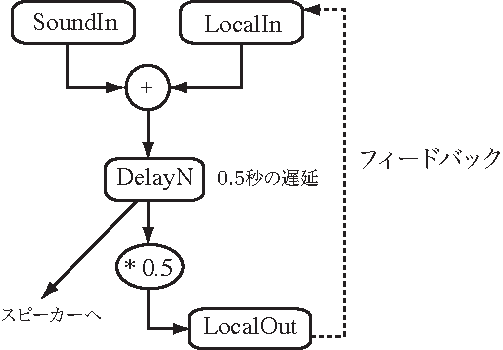
\includegraphics[scale=0.7]{feedback.pdf}
	\end{center}
	\label{フィードバック・ディレイの成り立ち}
\end{figure}

\begin{lstlisting}[caption=フィードバック・ディレイ, label=code:feedback]
{
	a = SoundIn.ar([0,1]) + LocalIn.ar(2);
	d = DelayN.ar(a, 0.5, 0.5);
	LocalOut.ar(d*0.5);
	d
}.play
\end{lstlisting}

\subsection{ピンポン・ディレイ}
フィードバック・ディレイにアレンジを加え、リスト\ref{code:pinpong}のように各ディレイが左右のスピーカーから交互に聞こえるようにすることもできる。

\begin{lstlisting}[caption=ピンポン・ディレイ, label=code:pingpong]
{
	i = SoundIn.ar(0) +  SoundIn.ar(1);
	d = DelayN.ar(i, 0.25, 0.25);
	l = LocalIn.ar(2);
	i = l[0] + i;
	d = l[1] + d;
	l = DelayN.ar(i, 0.5, 0.5) * 0.5; 
	r = DelayN.ar(d, 0.5, 0.5) * 0.5;
	LocalOut.ar([l,r]);
	[l,r+d]
}.play
\end{lstlisting}

リストでは2チャンネルのLocalIn/Outを使っている。4行目で、LocalInの引数の2を与え、オーディオ信号のArrayを取り出し、それぞれマイクからの入力音とマイク入力音を0.25秒遅延させたものに足している(5,6行目)。
そして、それぞれにDelayNと*0.5で個別に遅延と減衰処理を施しLocalOutとスピーカーに送っている。

\subsection{マルチタップ・ディレイ}
リスト\ref{code:multitap}のようにDelayNとArrayと組み合わせて、リズミカルなディレイを作る事も可能である。尚、このエフェクトはその性質上入力ソースがモノラルである必要があるため、2行目でステレオ入力信号を加算しモノラル化している。

\begin{lstlisting}[caption=マルチタップ・ディレイ, label=code:multitap]
{
	a = [1, 2, 4, 6, 7] * 0.1;
	Mix.ar(DelayN.ar(SoundIn.ar([0,1]), a, a));
}.play
\end{lstlisting}

このコードで変数aはマルチタップ・ディレイのリズムパターンが定義されたArrayが格納されている。Arrayは[1, 2, 4, 6, 7]というリズムパターンに0.1が掛けられているので、その内容は[0.1, 0.2, 0.4, 0.6, 0.7]となる、このArrayをDelayNの最大ディレイ・タイムとディレイ・タイムにそれぞれ適応している。このように引数にArrayが与えられた場合、SCは自動的にDelayNを複製する。ここでは5つの要素からなるArrayが与えられたためDelayNが5つ作られ、それぞれに異なった最大ディレイ・タイム及びディレイ・タイムが指定される。この全てのDelayNからの出力を{\bf Mix}というUgenを使って全て加算している。2行目の定数0.1を変更する事で、リズムを保持したまま、テンポだけを変える事が可能である。

\begin{itembox}[l]{Mix}
{\footnotesize 
{\it array}内の音声信号を全て加算する\\
.ar({\it array})\\
{\it array}$\cdots$音声信号のArray、全てのチャンネルが加算される\\
}
\end{itembox}

\section{リバーブ}
残響効果を入力音に加えるには、以下のようにFreeVerbというUgenを利用する。

\begin{lstlisting}[caption=リバーブ, label=code:reverb]
{
	FreeVerb.ar(SoundIn.ar([0,1]), 1.0);
}.play
\end{lstlisting}

\begin{itembox}[l]{FreeVerb}
{\footnotesize 
原音にリバーブ(残響効果)を付加するUgen

.ar({\it in}, {\it mix}, {\it room}, {\it damp}, {\it mul}, {\it add})\\

{\it in}$\cdots$入力信号\\
{\it mix}$\cdots$原音と加工音のバランス、1,0で加工音のみ、0.0で原音のみ\\
{\it room} $\cdots$ルームサイズ、1.0が最大、0.0が最小。\\
{\it damp} $\cdots$高周波数のダンプ。0から1の範囲で指定\\
}
\end{itembox}

\section{フィルタ}
SCには様々なフィルタが予め用意されている。リスト\ref{code:highpass}では、入力音にハイパス・フィルタを施し、3000Hz以下の低周波成分を減衰させている。

\begin{lstlisting}[caption=ハイパス・フィルタ, label=code:highpass]
{
	HPF.ar(SoundIn.ar([0,1]), 3000);
}.play
\end{lstlisting}

HPF(High Pass Filter) の他にもLPF(Low Pass Filter)、BPF(Band Pass Filter)、Moog、TwoPoleなど様々なフィルタが用意されている。「Filter」をヘルプで調べると、全てのフィルタのリストを見ることができる。

\begin{itembox}[l]{HPF}
{\footnotesize 
2次バターワース・ハイパスフィルタ
.ar({\it in}, {\it freq}, {\it mul}, {\it add})\\

{\it in}$\cdots$入力信号\\
{\it freq}$\cdots$カットオフ周波数\\
}
\end{itembox}

\section{ワウワウ}
リスト\ref{code:wahwah}では、バンド・パスフィルタ中央周波数のパラメータをLFOでコントロールすることにより、ファンク・ギターなどでお馴染みの「ワウワウ」のエフェクトを作成している。
\begin{lstlisting}[caption=ワウワウ, label=code:wahwah]
{
	l = SinOsc.ar(5, 0, 1000, 1500);
	BPF.ar(SoundIn.ar([0,1]), l, 0.5);
}.play。
\end{lstlisting}

BPFの三番目の引数はrq(reciprocal of Q)値であり、この値が少なければ少ないほどフィルタを通過する帯域幅が狭くなり、強くワウワウがかかる。

\begin{itembox}[l]{BPF}
{\footnotesize 
2次バターワース・バンドパスフィルタ
.ar({\it in}, {\it freq}, {\it rq}, {\it mul}, {\it add})\\

{\it in}$\cdots$入力信号\\
{\it freq}$\cdots$中央周波数\\
{\it rq}$\cdots$reciprocal of Q値\\
}
\end{itembox}

\section{自作エフェクタをSynthDefとしての定義する}
SC3ではこれまでに制作してきたエフェクターを組み合わせ、SynthDefとして定義することも可能である。リスト\ref{code:combination}ではディストーション・ディレイ・リバーブを連結して、より複雑なエフェクトを実装し、それを「myEffect」というSynthDefとして定義している。これにより、複数の作品で気に入ったエフェクタを再利用する事が用意となる。

\begin{lstlisting}[caption=エフェクトの組み合わせ, label=code:combination]
SynthDef("myEffect",{
	i = SoundIn.ar([0,1]);
	d = (i * 100).distort / 100 + d;
	d = DelayN.ar(d, 0.5, 0.5) + d;
	d = d + FreeVerb.ar(d, 1.0);
	Out.ar(0, d);
}).load;

Synth("myEffect")
\end{lstlisting}


\section{まとめ}
今回はSCによる様々なエフェクトのプログラミングを学習した。エフェクタは、さらにSCのバス(Bus)と言われる機能を利用して、エフェクタのSynthを複数繋ぐ、音を生成するSynthとエフェクタを定義したSynthを組み合わせて、自作シンセ音に各種エフェクトを
適応するという等、様々な応用が可能である。このバス機能については、また回を改めて紹介する。

\bibliographystyle{jplain}
\begin{thebibliography}{citations}
  \bibitem{scsite} {\it SuperCollider}, \url{http://supercollider.sourceforge.net}(アクセス日 2014年6月10日)
\end{thebibliography}

\section{著者プロフィール}
\subsection*{美山 千香士 (Chikashi Miyama)}
作曲家、電子楽器創作家、映像作家、パフォーマー。国立音楽大学音楽デザイン学科より学士・修士を、スイス・バーゼル音楽アカデミーよりナッハ・ディプロムを、アメリカ・ニューヨーク州立バッファロー大学から博士号を取得。Prix Destellos特別賞、ASCAP/SEAMUS委嘱コンクール2位、ニューヨーク州立大学学府総長賞、国際コンピュータ音楽協会賞を受賞。2004年より作品と論文が国際コンピュータ音楽会議に12回入選、現在までに世界19カ国で作品発表を行っている。 2011年、DAAD(ドイツ学術交流会)から研究奨学金を授与され、ドイツ・カールスルーエのZKMで客員芸術家として創作活動に従事。近著に「Pure Data-チュートリアル&リファレンス」(Works Corporation 社)がある。現在ドイツ・ケルン音楽大学講師。スイス・チューリッヒ芸術大学コンピュータ音楽・音響研究所(ICST)研究員。バーゼル造形大学のプロジェクト「Experimental Data Aesthetics」プログラマ。
\url{http://chikashi.net}

\end{document}
